\section*{Problem 8-2 Hierarchical Clustering}

\begin{figure}[h]
	\centering
	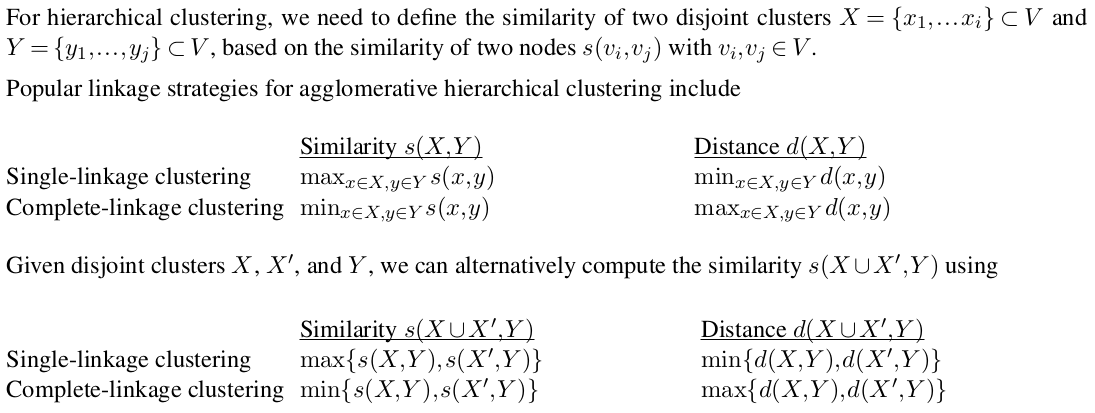
\includegraphics[width=0.9\linewidth]{content/problem2.png}
	\label{distribution}
\end{figure}

\begin{enumerate}
	\item Discuss why Single-linkage and Complete-linkage swap their definitions (i.e. $min$ and $max$) when used with a similarity rather than a distance function.
	\hrule \relax
	
	After the merge process of nodes into communities, there are three approaches for calculating the new similarities: single-linkage (take the maximum), complete-linkage (take the minimum) and average-linkage.
	If the distance between two nodes is small (min), the similarity is high (max). And vice versa if the distance between two nodes is high (max), the similarity is low (min). 
	Complete-linkage uses the maximum distance (which is the minimum similarity).
	Single-linkage uses the maximum similarity (which is the minimum distance).
	
	\hrule \relax
	\item Given the following similarity matrix $x^{o}_{ij}$ , based on the topological overlap (cf. slide 9-22), perform agglomerative hierarchical clustering, using single-linkage.
	
	\begin{equation}
		x^{o}_{ij} = \begin{blockarray}{ccccccc}
		A & B & C & D & E & F  \\
		\begin{block}{(cccccc)c}
		0 & 1 & 1/2 & 1 & 1 & 0 & A \\
		1 & 0 & 1/3 & 1 & 1 & 0 & B \\
		1/2 & 1/3 & 0 & 1/3 & 1/3 & 1 & C \\
		1 & 1 & 1/3 & 0 & 1 & 0 & D \\
		1 & 1 & 1/3 & 1 & 0 & 0 & E \\
		1/2 & 0 & 1 & 0 & 0 & 0 & F \\
		\end{block}
		\end{blockarray}
	\end{equation}
	
	Recall that for hierarchical clustering, you need to:
	\begin{itemize}
		\item Find the maximum similarity $s(i,j)$,
		\item Merge the corresponding clusters,
		\item Update the similarity matrix by merging rows/columns $i$ and $j$ according to the linking strategy.
	\end{itemize}

	Begin by assigning each node to a separate cluster (each node is its own cluster), and repeat the above procedure until only one cluster remains. Write out the similarity matrix after each iteration and draw the resulting dendrogram. During each iteration, multiple sets may have the same maximum similarity. In this case, you may still only merge two clusters at a time. In this case, also prefer the merge of two smaller clusters over a bigger one, i.e., prefer to merge two clusters with cardinality 1 over the merge of clusters with size 2 and size 1, respectively.
	
	\hrule \relax
	
	single-linking strategy: take the minimum value
	
	1. Merge A and B (maximum similarity 1)
	\begin{equation}
	x^{o}_{ij} = \begin{blockarray}{cccccc}
	A,B &  C & D & E & F  \\
	\begin{block}{(ccccc)c}
	0 & 1/3 & 1 & 1 & 0 & A,B \\
	1/3 & 0 & 1/3 & 1/3 & 1 & C \\
	1 & 1/3 & 0 & 1 & 0 & D \\
	1 & 1/3 & 1 & 0 & 0 & E \\
	0 & 1 & 0 & 0 & 0 & F \\
	\end{block}
	\end{blockarray}
	\end{equation}
	
	Cluster: (A,B),C,D,E,F
	
	2. Merge C and F (maximum similarity 1)
	\begin{equation}
	x^{o}_{ij} = \begin{blockarray}{ccccc}
	A,B &  C, F & D & E  \\
	\begin{block}{(cccc)c}
	0 & 0 & 1 & 1 & A,B \\
	0 & 0 & 0 & 0 & C,F \\
	1 & 0 & 0 & 1 & D \\
	1 & 0 & 1 & 0 & E \\
	\end{block}
	\end{blockarray}
	\end{equation}
	
	Cluster: (A,B),(C,F),D,E
	
	3. Merge D and E (maximum similarity 1)
	\begin{equation}
	x^{o}_{ij} = \begin{blockarray}{cccc}
	A,B &  C,F & D,E  \\
	\begin{block}{(ccc)c}
	0 & 0 & 1 & A,B \\
	0 & 0 & 0 & C,F \\
	1 & 0 & 0 & D,E \\
	\end{block}
	\end{blockarray}
	\end{equation}
	
	Cluster: (A,B),(C,F),(D,E)
	
	4. Merge (A,B) and (D,E) (maximum similarity 1)
	\begin{equation}
	x^{o}_{ij} = \begin{blockarray}{ccc}
	A,B,D,E  &  C,F \\
	\begin{block}{(cc)c}
	0 & 0 & A,B,D,E \\
	0 & 0 & C,F \\
	\end{block}
	\end{blockarray}
	\end{equation}
	
	Cluster: (A,B,D,E),(C,F)
	
	5. Merge (A,B,D,E) and (C,F) (maximum similarity 1/3)
	
	results in one cluster containing all nodes
	
	Cluster: (A,B,D,E,C,F)
	
	Dendrogram:
	
	\begin{tikzpicture}[sloped]
	\node (A) at (-6,0) {A};
	\node (B) at (-4,0) {B};
	\node (D) at (-2,0) {D};
	\node (E) at (0,0) {E};
	\node (C) at (2,0) {C};
	\node (F) at (4,0) {F};
	\node (AB) at (-5,1) {};
	\node (DE) at (-1,1) {};
	\node (CF) at (3,1) {};
	\node (ABDE) at (-3,2) {};
	\node (all) at (0,3) {};
	
	\draw  (A) |- (AB.center);
	\draw  (B) |- (AB.center);
	\draw  (D) |- (DE.center);
	\draw  (E) |- (DE.center);
	\draw  (C) |- (CF.center);
	\draw  (F) |- (CF.center);
	\draw  (AB.center) |- (ABDE.center);
	\draw  (DE.center) |- (ABDE.center);
	\draw  (CF.center) |- (all.center);
	\draw  (ABDE.center) |- (all.center);
	
	\draw[->] (-7,0) -- node[above]{distance} (-7,4);
	\end{tikzpicture}
	
	\hrule \relax
\end{enumerate}